\documentclass{article}
\usepackage[T1]{fontenc}
\usepackage{lmodern}
\usepackage{graphicx}
\usepackage{amsmath,amssymb}
\usepackage[a4paper,margin=2cm]{geometry}
\usepackage[absolute,overlay]{textpos}
\setlength{\TPHorizModule}{1mm}
\setlength{\TPVertModule}{1mm}
\usepackage[indonesian]{babel}
\usepackage{hyperref}
\setlength{\emergencystretch}{2em}
% unit: Halaman 22

\begin{document}

% === Halaman 22 (llm) ===

\vspace{83.16mm}

ShiftRows()

% deskripsi: Ilustrasi operasi ShiftRows pada matriks state dalam algoritma AES, menunjukkan pergeseran baris secara siklik ke kiri.
% bbox normalisasi: [0.1600, 0.2700, 0.8200, 0.5500]
\begin{textblock*}{138.60mm}(33.60mm,80.19mm)
\noindent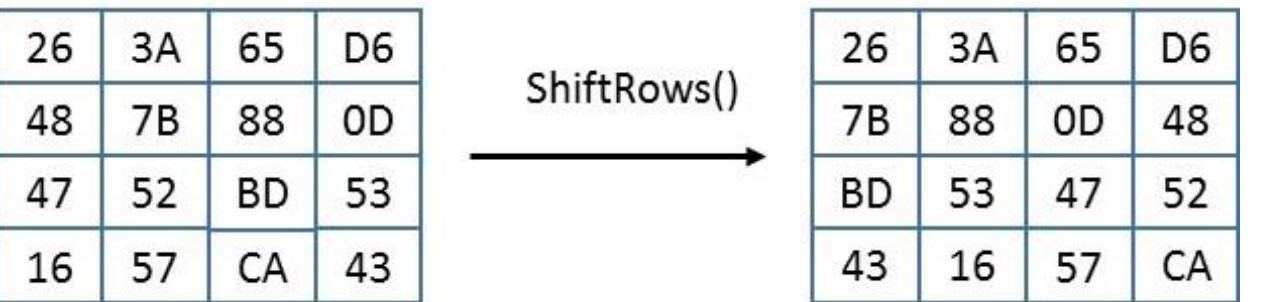
\includegraphics[width=138.60mm,height=83.16mm]{../../images/llm/page_022_img_01.png}%
\end{textblock*}

\end{document}
